\subsection{Virtual Displacements and the Birth of the Euler-Lagrange Equation}

This led him into the territory of what we now call \textbf{variational calculus} — a kind of calculus where the unknowns are not just numbers or functions, but entire paths and trajectories. It was here that Lagrange made his most profound contribution: a symbolic recipe to determine the true path of motion, not by tracing it directly, but by ruling out all the alternatives.

At the heart of this approach is a quantity called the \textit{Lagrangian}, which captures a system’s energetic balance:

\[
L = T - V
\]

the kinetic energy minus the potential energy.

\medskip

\begin{HistoricalSidebar}{Lagrange and the Calculus of the Best Possible World}
    
        \textbf{Gottfried Wilhelm Leibniz} (1646–1716) believed that the universe was a rational, optimized system—created by a perfect God who chose the \textbf{best of all possible worlds}. For Leibniz, this meant that nature always followed the most elegant, efficient paths. Every event had a sufficient reason, and every motion unfolded with mathematical necessity.
    
        \medskip
    
        This vision wasn’t just theological—it was mathematical. Leibniz imagined a cosmos that could be described in terms of \textbf{infinitesimals, differentials, and minima}, governed by the principle that nature “does nothing in vain.” These ideas laid the philosophical and technical groundwork for the development of calculus, and they would find their purest mechanical expression in the work of \textbf{Joseph-Louis Lagrange}.
    
        \medskip
    
        In his 1788 masterpiece, \textit{Mécanique Analytique}, Lagrange reformulated Newtonian mechanics using only algebra and calculus, eliminating the need for geometric diagrams or direct references to physical forces. Instead, he treated the evolution of physical systems as an \textbf{optimization problem}—exactly the kind of principle Leibniz had championed.
    
        \medskip
    
        Lagrange’s use of the \textbf{principle of least action}—that nature selects the path which minimizes (or extremizes) a certain quantity—was a direct echo of Leibniz’s metaphysics. In Lagrange’s mechanics, the universe behaves not like a machine of levers and weights, but like a system solving an elegant equation: \textbf{minimal effort, maximal coherence}.
    
        \medskip
    
        \textbf{Quote from Leibniz (1697):}
        \begin{quote}
        “In the effects of nature, the greatest variety is brought about with the greatest order; and this is the mark of divine wisdom.”
        \end{quote}
    
        Leibniz dreamed of a universe governed by calculus. Lagrange wrote the equations that made it move.
    
\end{HistoricalSidebar}

\medskip

The idea of a \textit{virtual displacement} predates Lagrange, going back to the principle of \textit{virtual work} used by early mechanicians like Galileo, Torricelli, and the Bernoulli brothers. These were imagined shifts—not real motions—tiny hypothetical nudges you could apply to a system in equilibrium to see how the forces would respond.

Lagrange took that idea and breathed motion into it.

He reinterpreted these imaginary displacements as probes—not of static balance, but of dynamic possibility. What if, he asked, we could apply a small tweak — not to the forces, but to the \textit{path itself}? What if nature picks the path where these imagined variations make no first-order difference?

That “path” is governed by a quantity called the \textit{action}, the time-integral of the Lagrangian \( L = T - V \). And Lagrange’s insight was this:

\begin{quote}
\textit{Among all the possible ways the system could evolve, nature picks the one for which the action is stationary.}
\end{quote}

Not minimal. Not maximal. Just stationary — like standing still at the crest of a hill.

\medskip

\begin{HistoricalSidebar}{The Principle of Virtual Work}
  Long before the age of Lagrange, mechanicians had recognized that you could probe a system’s balance by imagining “infinitesimal” shifts.  In the early 17\textsuperscript{th} century, Galileo—while studying the lever—implicitly used virtual displacements to compare weights and distances.  Evangelista Torricelli and the Bernoulli brothers (particularly Johann and Jakob) extended the idea to fluids and elastic systems, noting that an imagined nudge at equilibrium yields no net “virtual work.”  

  \medskip

  Lagrange would later embrace this dynamic virtual work, recasting it into his variational calculus and showing that the true path makes the \emph{action} stationary.  Thus, what began as a static balancing trick became the cornerstone of analytical mechanics.
\end{HistoricalSidebar}

\subsection{The Birth of Kinetic Energy}
By the late 17\textsuperscript{th} century, Leibniz had already introduced the notion of \emph{vis viva} (\(m\,v^2\)) as a measure of a body’s living force.  Euler, working in the language of Cartesian coordinates \((x,y,z)\), recognized that for a mass \(m\) whose position varies in time as \(x(t),y(t),z(t)\), the quantity

\[
T
\;=\;
\tfrac12\,m\!\bigl[\dot x^2+\dot y^2+\dot z^2\bigr]
\quad\bigl(\dot x\equiv\tfrac{dx}{dt}\bigr)
\]

has exactly the dimensions of work and composes additively in elastic collisions.  This “one half mass times speed squared” form thus became the canonical expression for kinetic energy.

\medskip

\begin{HistoricalSidebar}{The Vis Viva Debate}
  Long before “energy” entered the textbooks, Gottfried Wilhelm Leibniz proposed in the 1680s that what he called \emph{vis viva}—literally “living force”—was the true invariant of motion.  In his \emph{Essais de Théodicée} (1686) and later in the unpublished \emph{Hypothesis Physica Nova}, Leibniz argued that in elastic collisions the sum of \(m\,v^2\) (not \(m\,v\)) remains constant.  

  \medskip
  
  This claim flew in the face of Cartesian mechanics, which tracked momentum (\(\sum m\,v\)) and envisioned bodies as inert; instead, Leibniz insisted that motion carried a dynamic “force” proportional to velocity squared.  His friend Johann Bernoulli quickly adopted the idea, applying it to pendulums and early orbital approximations.  Critics like Christiaan Huygens and the Cartesians objected, pointing to confusing units and collision experiments that seemed to support simpler momentum conservation.  

  \medskip
  
  The debate raged until Émilie du Châtelet’s 1740 translation and commentary on Newton’s \emph{Principia} rehabilitated vis viva by clarifying its relation to work and potential.  By the turn of the 19th century, with Coriolis and Rankine formalizing “kinetic energy” as \(\tfrac12\,m\,v^2\), Leibniz’s living force found its rightful place at the heart of analytical mechanics.
\end{HistoricalSidebar}


\subsection{The Emergence of Potential Energy}

To capture the work stored by position alone, 18\textsuperscript{th}-century mechanics defined a function \(V(x,y,z)\) whose infinitesimal change exactly balances the work done by the force components \(F_x,\,F_y,\,F_z\).  In coordinate form one writes

\[
dV
\;=\;
-\,\bigl(F_x\,dx \;+\;F_y\,dy \;+\;F_z\,dz\bigr),
\]

so that, choosing some reference point \((x_0,y_0,z_0)\),

\[
V(x,y,z)
=
-\,\int_{x_0}^{x}F_x(\xi,y_0,z_0)\,d\xi
\;-\;
\int_{y_0}^{y}F_y(x,\eta,z_0)\,d\eta
\;-\;
\int_{z_0}^{z}F_z(x,y,\zeta)\,d\zeta.
\]

\medskip

\begin{HistoricalSidebar}{Dummy Variables in Multivariable Integration}
    When Leibniz invented the integral “\(\displaystyle\int\)” in the 1670s, he paired it with a differential “\(dx\)” to mark summation over a single coordinate.  By the mid-18\textsuperscript{th} century, Euler and his followers were already extending this to functions of several variables, introducing symbols like \(\xi,\eta,\zeta\) to avoid confusion in triple and higher-order integrals.
    
    \medskip
    
    In early multivariable practice one writes, for example, the work-integral along the \(x\)-axis as

    \[
    \int_{x_0}^{x} F_x(\xi,y_0,z_0)\,d\xi,
    \]

    where \(\xi\) is a \emph{dummy variable} running from the reference point \(x_0\) to \(x\), while \(y\) and \(z\) remain fixed at \(y_0,z_0\).  Likewise, one uses \(\eta\) for the \(y\)-integral and \(\zeta\) for the \(z\)-integral:

    \[
    \int_{y_0}^{y} F_y(x,\eta,z_0)\,d\eta,
    \quad
    \int_{z_0}^{z} F_z(x,y,\zeta)\,d\zeta.
    \]
    
    \medskip
    
    By the 19\textsuperscript{th} century Cauchy and his successors formalized “bound” versus “free” variables: any symbol appearing inside an integral and its differential (like \(\xi\) in \(\int f(\xi)\,d\xi\)) has no identity outside that integral.  In multivariable work integrals, \(\xi,\eta,\zeta\) simply keep track of which coordinate is being “summed over”—they’re purely bookkeeping, and one is free to rename them without changing the value:
    \[
    \int_{x_0}^{x}F_x(\xi,\dots)\,d\xi
    =
    \int_{x_0}^{x}F_x(s,\dots)\,ds.
    \]
    
    \medskip
    
    Today, when we write

    \[
    V(x,y,z)
    =
    -\,\int_{x_0}^{x}F_x(\xi,y_0,z_0)\,d\xi
    \;-\;
    \int_{y_0}^{y}F_y(x,\eta,z_0)\,d\eta
    \;-\;
    \int_{z_0}^{z}F_z(x,y,\zeta)\,d\zeta,
    \]

    we rely on that centuries-old convention: \(\xi,\eta,\zeta\) are dummy variables that guide each one-dimensional slice of the three-dimensional integral.
    \end{HistoricalSidebar}
    

\medskip

With these definitions in hand, one sees that

\[
V(x,y,z)
=
-\,\int_{x_0}^{x}F_x(\xi,y_0,z_0)\,d\xi
\;-\;
\int_{y_0}^{y}F_y(x,\eta,z_0)\,d\eta
\;-\;
\int_{z_0}^{z}F_z(x,y,\zeta)\,d\zeta,
\]

is simply the total work required to move the mass from \((x_0,y_0,z_0)\) to \((x,y,z)\) along that three‐step path.  

Armed with

\[
T=\tfrac12\,m\bigl(\dot x^2+\dot y^2+\dot z^2\bigr),
\qquad
V=V(x,y,z),
\]

Lagrange could then form the Lagrangian 

\[
L(x,y,z,\dot x,\dot y,\dot z)\;=\;T-V
\]

and—with his new calculus of variations—derive the Euler–Lagrange equations without ever drawing a single force-diagram.

\subsection{Reading the Equation Qualitatively}

Let’s unpack what this equation really says.

\[
\frac{d}{dt} \biggl( \frac{dL}{d\dot{q}_i} \biggr) \;-\;\frac{dL}{dq_i} \;=\; 0
\]

Here we capture in one compact line what once required separate integrals and dummy variables (\(\xi,\eta,\zeta\)) for each coordinate direction.  Instead of writing out three work‐integrals

\[
-\,\int_{x_0}^{x}F_x(\xi,y_0,z_0)\,d\xi
\;-\;
\int_{y_0}^{y}F_y(x,\eta,z_0)\,d\eta
\;-\;
\int_{z_0}^{z}F_z(x,y,\zeta)\,d\zeta,
\]

the Euler–Lagrange equation bundles all of those conditions into a single variational statement.

The term \(\displaystyle \frac{dL}{d\dot{q}_i}\) measures how the Lagrangian changes when we tweak the velocity of the coordinate \(q_i\).  This is the \emph{generalized momentum}.

The derivative \(\displaystyle \frac{d}{dt}\!\bigl(\tfrac{dL}{d\dot{q}_i}\bigr)\) shows how that momentum evolves over time—like a generalized force.

The term \(\displaystyle \frac{dL}{dq_i}\) captures how the system’s energy changes when we nudge its position.

Together, the equation says: these two tendencies—momentum’s change and the pull from position—must exactly balance, all in one neat package.

\begin{quote}
    \textit{The path nature chooses is one where the push from motion and the pull from position are always in perfect balance.}
\end{quote}

Moreover, by labeling the generalized coordinates as \(q_1,\dots,q_n\) and letting \(i\) run from 1 to \(n\), this single concise statement

\[
\frac{d}{dt}\Bigl(\frac{dL}{d\dot{q}_i}\Bigr)-\frac{dL}{dq_i}=0
\]

immediately extends to systems of \emph{arbitrary} dimension.  

This is the \textbf{Euler-Lagrange equation}, though it was Lagrange who first wrote it down.

\medskip

\begin{HistoricalSidebar}{From Partial Derivatives to the Gradient Operator}
    Centuries before the nabla symbol “\(\nabla\)” became standard, Lagrange and his peers probed how a system’s energy shifts with position by taking partial derivatives of the Lagrangian:
    
    \[
    \frac{\partial L}{\partial q_i}
    \]
    
    This notation expresses the infinitesimal change in \(L\) when the generalized coordinate \(q_i\) is nudged, without yet grouping those individual derivatives into a single vector form.

    \medskip
    
    In the late 18\textsuperscript{th} century, mathematicians like Euler and Lagrange routinely worked coordinate by coordinate—Cartesian or otherwise—using separate partials to capture spatial variation.  The concept of a unified “gradient” was implicit but unwritten.

    \medskip
    
    It was only in the 1830s that William Rowan Hamilton introduced the nabla symbol to represent the collection of all partial derivatives in one operator, and later Peter Guthrie Tait and Lord Kelvin solidified its role in their \textit{Treatise on Natural Philosophy}.  Looking back, Lagrange’s simple \(\partial L/\partial q_i\) entries can be seen as early hints of this powerful unification, laying groundwork for the gradient operator we now use to describe fields and forces in multidimensional spaces.
\end{HistoricalSidebar}








\subsection{From Variations to Equations}

By imagining small variations \( \delta q_i(t) \) to the coordinate functions \( q_i(t) \), and requiring that the start and end points stay fixed, Lagrange asked how the action \( S = \int L\,dt \) would change. The requirement that the action be stationary under all such variations leads directly to:

\[
\frac{d}{dt} \left( \frac{dL}{d\dot{q}_i} \right) - \frac{dL}{dq_i} = 0
\]

From a single principle — not based on force, but on energetic preference — emerged a universal law of motion. One that could describe systems without ever drawing a single diagram.

Lagrange called these variations “virtual” to emphasize that they are imagined alternatives, not real motions. We don’t change the trajectory physically — we change it in thought, asking whether any nearby path might yield a different outcome. If not — if the action remains stationary — then we’ve found nature’s chosen trajectory.

It was a subtle but radical shift:
\begin{quote}
    \textit{From “What causes what?” to “What path would resist all alternatives?”}
\end{quote}

\subsection{The Spirit of Determinism}

The Lagrangian method captured the Enlightenment dream: a physics of perfect predictability. Every system, no matter how complex, could be described not by what happens, but by what \textit{must} happen, according to laws derived from symmetry, structure, and principle.

Where Newton saw objects being pushed and pulled, Lagrange saw trajectories preordained by the internal logic of energy. It was a vision of the cosmos as a deterministic scroll, already written — with the Euler-Lagrange equation as its grammar.

\begin{quote}
    \textit{Nature explores all the paths it could take — and chooses the one where the story is already most coherent.}
\end{quote}


\begin{HistoricalSidebar}{Fermat and the Wisdom of Light}

    In the 1600s, while Descartes was busy mathematizing the heavens and Galileo was redefining motion, \textbf{Pierre de Fermat} made a deceptively simple observation about something far less massive: \emph{light}.

    \medskip
    
    Fermat proposed what would become known as the \textbf{Principle of Least Time}: \emph{light always travels between two points along the path that takes the least time}. It wasn’t just a guess—it matched experimental results, especially the strange bending of light as it passed from air into water.

    \medskip
    
    While Descartes had explained refraction using the force of impact, Fermat took a different route. He calculated the path a light ray would take if it "chose" the fastest route—slower in water, faster in air—and astonishingly, this mathematical minimum exactly matched what nature actually did.

    \medskip
    
    In other words, Fermat believed the universe was lazy in a profoundly elegant way: it always optimized.
    
    \medskip
    
    A century later, \textbf{Joseph-Louis Lagrange} would elevate this idea into a new language entirely: the \textbf{calculus of variations}. Instead of just light, Lagrange applied it to the motion of \emph{everything}. Why do planets move the way they do? Because their paths make the action minimal. Why does a pendulum swing the way it does? Same reason. Just as Fermat’s light found the quickest path, Lagrange’s mechanics found the most efficient one—mathematically encoded as the path that extremizes a function called the \textit{Lagrangian}.

    \medskip
    
    Thus, Fermat’s humble ray of light cast a long shadow—one that reached all the way into the foundations of modern physics.
    
\end{HistoricalSidebar}

   





\subsection{Generalized Coordinates in Lagrange’s Mechanics}

Lagrange showed that for a system with \(n\) independent variables \(q_1,\dots,q_n\), one may regard the Lagrangian as a function of the coordinates, their time-rates, and time itself:
\[
L \;=\; L\bigl(q_1,\dots,q_n,\;q_1',\dots,q_n',\;t\bigr),
\]
where \(q_i'=\tfrac{dq_i}{dt}\).  He then used the notation
\[
\frac{dL}{dq_i}
\quad\text{and}\quad
\frac{dL}{dq_i'},
\]
to mean “how \(L\) changes when \(q_i\) alone is varied” and “how \(L\) changes when \(q_i'\) alone is varied,” holding all other \(q_k\) and \(q_k'\) constant.

Applying his variational recipe to each coordinate \(q_i\), Lagrange arrived at a set of \(n\) equations of motion, one for each \(i=1,\dots,n\):
\[
\frac{d}{dt}\!\Bigl(\frac{dL}{dq_i'}\Bigr)
\;-\;
\frac{dL}{dq_i}
\;=\;
0.
\]
With this compact algebraic rule, he replaced the old Cartesian force-balance methods by a unified system of equations—without ever invoking partial derivatives or modern manifold concepts.  



\subsection{Lagrange’s Coordinate–Velocity Space}

Rather than work solely with positions or forces, Lagrange treated each instantaneous state of a system as a point in a “coordinate–velocity space.”  For a system with \(n\) degrees of freedom, one records
\[
\bigl(q_1,\dots,q_n;\;q_1',\dots,q_n'\bigr),
\]
where \(q_i\) is the generalized coordinate and \(q_i'=\tfrac{dq_i}{dt}\) its time‐rate.  This \(2n\)-tuple uniquely fixes both where the system is and how it is moving.

\medskip

On this space Lagrange defined his function
\[
L\bigl(q_1,\dots,q_n;\;q_1',\dots,q_n';\;t\bigr)
\;=\;
T-V,
\]
assigning to each point the difference of kinetic and potential energy.  A motion of the system then becomes a curve
\[
t\;\longmapsto\;\bigl(q_i(t),\,q_i'(t)\bigr)
\]
in this space, and the true motion is singled out by the requirement that the integral of \(L\) along the curve be stationary.

\medskip

Viewed in this way, Lagrange’s method unifies position and velocity into one arena: every equation of motion emerges from the single variational principle applied to \(L\) on the full coordinate–velocity space.  


\begin{figure}[H]
    \centering
    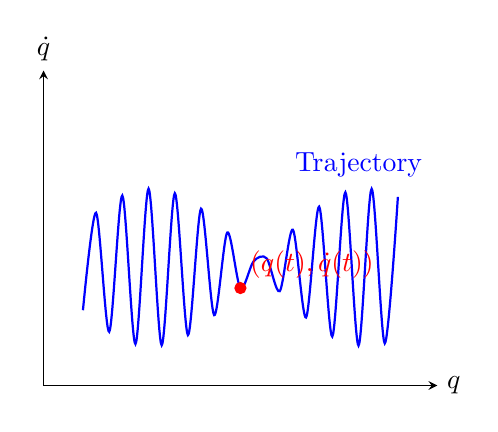
\begin{tikzpicture}[>=stealth, scale=1]
      % Axes
      \draw[->] (0,0) -- (5,0) node[right] {$q$};
      \draw[->] (0,0) -- (0,4) node[above] {$\dot q$};
      % Trajectory curve
      \draw[thick, domain=0.5:4.5, smooth, variable=\t, blue]
        plot ({\t}, {1.5 + 1*sin(20*\t r)});
      % Mark a point on the trajectory
      \coordinate (P) at (2.5,{1.5 + sin(20*2.5 r)});
      \filldraw[red] (P) circle (2pt)
        node[above right] {$(q(t),\dot q(t))$};
      % Label the curve
      \node[blue] at (4,2.8) {Trajectory};
    \end{tikzpicture}
    \caption{Illustration of a curve in Lagrange’s coordinate–velocity space for a single degree of freedom.}
\end{figure}




\subsection{Kepler’s Second Law in \emph{(r,\(\theta\))} Configuration Space}

In Lagrange’s formulation, the motion of a planet under a central force can be viewed as a path in the two-dimensional configuration space with coordinates \((r,\theta)\).  The Lagrangian for a mass \(m\) orbiting a central body of mass \(M\) is

\[
L(r,\dot r,\dot\theta)
=\tfrac12\,m\bigl(\dot r^2 + r^2\dot\theta^2\bigr)
\;+\;\frac{G\,M\,m}{r},
\]

and since \(\theta\) does not appear explicitly in \(L\), the corresponding “generalized momentum”

\[
p_\theta \;=\; \frac{dL}{d\dot\theta} \;=\; m\,r^2\,\dot\theta
\]

is conserved.  But geometrically \(r^2\dot\theta\) is twice the areal velocity \(dA/dt\), so

\[
r^2\,\dot\theta \;=\;\text{constant}
\quad\Longrightarrow\quad
\frac{dA}{dt}=\tfrac12\,r^2\dot\theta=\text{constant},
\]

which is exactly Kepler’s Second Law: \emph{equal areas in equal times}.  

\begin{figure}[H]
\centering
\begin{tikzpicture}[>=stealth, xscale=0.02, yscale=1]
  % Axes
  \draw[->] (0,0) -- (370,0) node[right] {$\theta$ (deg)};
  \draw[->] (0,0) -- (0,4) node[above] {$r(\theta)$};
  % Elliptical orbit in (r,theta) space: r = a(1−e²)/(1+e cos θ), here a=3, e=0.5
  \draw[thick,domain=0:360,smooth,samples=200,blue]
    plot (\x,{2.25/(1+0.5*cos(\x))});
  % Mark aphelion and perihelion
  \filldraw[red] (180,{2.25/(1+0.5*cos(180))}) circle (2pt)
    node[above right] {aphelion};
  \filldraw[red] (0,{2.25/(1+0.5*cos(0))}) circle (2pt)
    node[below right] {perihelion};
  % Label curve
  \node[blue] at (200,3.2) {$(r(\theta),\theta)$};
\end{tikzpicture}
\caption{An elliptical orbit represented as a curve in the \((r,\theta)\) configuration space, where \(r(\theta)=\tfrac{a(1-e^2)}{1+e\cos\theta}\).}
\end{figure}



\begin{figure}[H]
    \centering
    % First (Cartesian) illustration
    \subcaptionbox{Ellipse in Cartesian $(x,y)$ plane\label{fig:ellipse-cartesian}}{%
      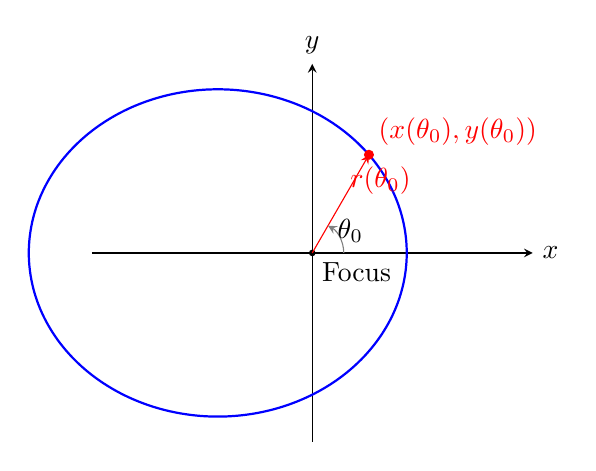
\begin{tikzpicture}[>=stealth,scale=0.8]
        % Axes
        \draw[->] (-3.5,0) -- (3.5,0) node[right] {$x$};
        \draw[->] (0,-3) -- (0,3) node[above] {$y$};
        % Elliptical orbit
        \draw[thick,blue,domain=0:360,smooth,samples=200]
          plot ({(2.25/(1+0.5*cos(\x)))*cos(\x)},
               {(2.25/(1+0.5*cos(\x)))*sin(\x)});
        % Focus
        \fill (0,0) circle (1.5pt) node[below right] {Focus};
        % Sample point at θ₀=60°
        \coordinate (P) at ({1.8*cos(60)},{1.8*sin(60)});
        \filldraw[red] (P) circle (2pt) node[above right] {$(x(\theta_0),y(\theta_0))$};
        % Radius vector
        \draw[red,->] (0,0) -- (P) node[midway,above right] {$r(\theta_0)$};
        % Angle arc
        \draw[->,gray] (0.5,0) arc[start angle=0,end angle=60,radius=0.5];
        \node at ({0.7*cos(30)},{0.7*sin(30)}) {$\theta_0$};
      \end{tikzpicture}
    }
    
    \vspace{1em}
    
    % Second (configuration‐space) illustration
    \subcaptionbox{Configuration‐space plot $r$ vs.\ $\theta$\label{fig:ellipse-rt}}{%
      \begin{tikzpicture}[>=stealth,xscale=0.02,yscale=1]
        % Axes
        \draw[->] (0,0) -- (370,0) node[right] {$\theta$ (deg)};
        \draw[->] (0,0) -- (0,4)   node[above] {$r(\theta)$};
        % r(θ) curve
        \draw[thick,blue,domain=0:360,smooth,samples=200]
          plot (\x,{2.25/(1+0.5*cos(\x))});
        % Sample point at (60,1.8)
        \filldraw[red] (60,1.8) circle (2pt) node[above right] {$(\theta_0,r(\theta_0))$};
        % Guides
        \draw[gray,dashed] (60,0) -- (60,1.8) -- (0,1.8);
      \end{tikzpicture}
    }
    
    \caption[Cartesian and $(r,\theta)$ views of an ellipse]{%
    Left: the physical orbit in the $(x,y)$ plane, drawn from the focus at the origin, with a sample radius vector $r(\theta_0)$.  
    Right: the corresponding curve in $(r,\theta)$ configuration space, showing how the same angle $\theta_0$ maps to the radial distance $r(\theta_0)$.}
\end{figure}
    